% !Mode:: "TeX:UTF-8"
% !TEX program  = xelatex
\title{What Angle Should We Throw a Football for Maximum Range}
\author[Iydon]{Iydon at DataHub}
\date{\today}
\institute[SUSTech]{
    Department of Mathematics \\
    Southern University of Science and Technology
}

\begin{frame}
	\maketitle
\end{frame}



\section{Introduction}
\begin{frame}[t]{Projectile Motion}
    \begin{block}{Projectile motion}
        Projectile motion is a form of motion experienced by an object or particle (a projectile) that is thrown near the Earth’s surface and moves along a curved path under the action of gravity only\footnote{In particular, the effects of air resistance are assumed to be negligible.}.
    \end{block}
\end{frame}

\begin{frame}{Projectile Motion}
    \begin{figure}
        \centering
        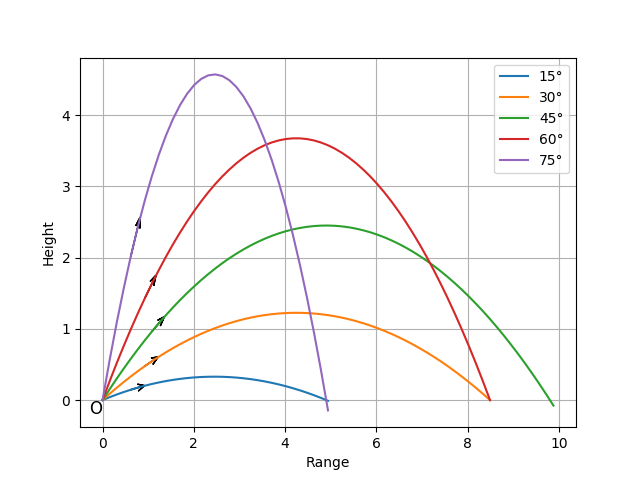
\includegraphics[width=.7\textwidth]{../figures/quadratic_equation-1.png}
        \caption{Parabolic trajectories at different angles}
    \end{figure}
\end{frame}



\section{Quadratic Equation}
\begin{frame}[t]{Definition}
    \begin{block}{Quadratic equation}
        In algebra, a quadratic equation (from the Latin \emph{quadratus} for ``square'') is any equation having the form
        \begin{equation}\label{E:1}
            c_2 x^2 + c_1 x + c_0 = 0,
        \end{equation}
        where $x$ represents an unknown, and $c_n$ ($n=0,1,2$) represent known numbers, with $a\neq 0$. If $a=0$, then the equation is linear, not quadratic, as there is no $c_2 x^2$ term. Then we can divide both sides of the equation by $c_2$, and replace $c_1/c_2$ with $b$, $c_0/c_2$ with $c$.
        \begin{equation}\label{E:quadratic-equation}
            x^2 + bx + c = 0.
        \end{equation}
        That is, every quadratic equation can be transformed into the form of Equation~\eqref{E:quadratic-equation}.
    \end{block}
\end{frame}

\begin{frame}[t]{Quadratic Formula and Its Derivation}
    \begin{equation}\label{E:quadratic-formula-1}
        \begin{aligned}
            x^2 + bx + c &= 0 \\
            x^2 + 2\frac{b}{2}x &= -c \\
            \left(x+\frac{b}{2}\right)^2 &= \frac{b^2-4c}{4}.
        \end{aligned}
    \end{equation}
    
    The left side of the Equation~\eqref{E:quadratic-formula-1} is a squared form, which means that it may have multiple solutions. That is, if $b^2-4c\geq 0$,
    \begin{equation}\label{E:quadratic-formula-2}
        \begin{aligned}
            x + \frac{b}{2} &= \pm \frac{\sqrt{b^2-4c}}{2} \\
            x &= \frac{-b\pm\sqrt{b^2-4c}}{2}.
        \end{aligned}
    \end{equation}
\end{frame}



\section{Applications}
\begin{frame}[t]{Solution to Article Title}
    \begin{figure}
        \centering
        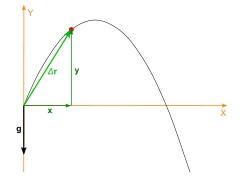
\includegraphics[width=.5\textwidth]{../figures/quadratic_equation-3.png}
        \caption{Parabolic trajectories at different angles}
    \end{figure}
\end{frame}

\begin{frame}[t]{Solution to Article Title}
    we have both horizontal and vertical distance at time $t$,
    \begin{equation}\label{E:solution-2}
        \begin{cases}
            S_x &= V\cos(\theta)t \\
            S_y &= V\sin(\theta)t - \frac{1}{2} gt^2
        \end{cases}
    \end{equation}

    We can find all of the coordinate $(S_x, S_y)$ with angle $\theta$. From Equation~\eqref{E:solution-2}, we have $t=\tfrac{2V\sin(\theta)}{g}$, then we substitute the expression of $t$ back to the $S_y$, we have the quadratic equation
    \begin{equation}\label{E:solution-3}
        S_y = \tan(\theta)S_x - \frac{g}{2V^2\cos^2(\theta)}S_x^2.
    \end{equation}

    From quadratic formula, we can solve this quadratic equation, the solutions are $0$ and $\tfrac{2V^2}{g}\sin(\theta)$. Obviously, $0$ is the initial position, then the football will land at $\tfrac{2V^2}{g}\sin(\theta)$, that is, $\tfrac{V^2}{g}\sin(2\theta)$.
\end{frame}

\begin{frame}[t]{Simulation of Projectile Motion}
    \begin{block}{}
        You can use quadratic equation to simulate projectile motion, which can solve free fall problems. If you are familiar with Python, you can use Python to draw the pictures of trajectories, and you will find it easy to use Python to solve quadratic equations, especially in symbolic calculations. And the code is in appendix of article.
    \end{block}
\end{frame}



\section{Conclusions}
\begin{frame}[t]{Conclusions}
    \begin{block}{}
        From this article, we introduce projectile motion and quadratic equation through a real world problem --- \emph{what angle should we throw a football for maximum range}, then we give a proper and accurate definition of quadratic equation, from which we derive quadratic formula for solving quadratic equations. Furthermore, we list some useful applications of the quadratic equation and implement them in \texttt{Python}.
    \end{block}
\end{frame}



\section*{Acknowledgments}
\begin{frame}[t]{Acknowledgments}
    \begin{itemize}
        \item The author would like to thank the Associate Editor and one referee for their valuable comments which have greatly improved the paper.
        \item The author’s research is fully supported by the DataHub Organization of China (No. 1000001).
    \end{itemize}
\end{frame}

\begin{frame}{Acknowledgments}
    \centering\Huge Thank you!
\end{frame}



\section*{References}
\begin{frame}[t]{References}
	\begin{thebibliography}{9}\large
        \bibitem{C:1} Wikipedia contributors. Projectile motion — Wikipedia, the free encyclopedia[EB/OL]. 2019. \url{https://en.wikipedia.org/w/index.php?title=Projectile_motion&oldid=928426750}.
        \bibitem{C:2} Wikipedia contributors. Trajectory — Wikipedia, the free encyclopedia[EB/OL]. 2019. \url{https://en.wikipedia.org/w/index.php?title=Trajectory&oldid=929280103}.
        \bibitem{C:3} Wikipedia contributors. Quadratic equation — Wikipedia, the free encyclopedia [EB/OL]. 2019. \url{https://en.wikipedia.org/w/index.php?title=Quadratic_equation&oldid=929716375}.
    \end{thebibliography}
\end{frame}
